% <- percent signs are used to comment
\documentclass[12pt]{article}

%%%%%% PACKAGES - this part loads additional material for LaTeX %%%%%%%%%
% Nearly anything you want can be done in LaTeX if you load the right package 
% (search ctan.org or google it if you are looking for something).  We will load
% here a few that we need for this document or that we expect you to need later.

% The next 3 lines are needed to fix shortcomings of TeX that only make sense given its 40-year history ...
% Simple keep and ignore.
\usepackage[utf8]{inputenc}
\usepackage[T1]{fontenc}
\usepackage{lmodern}
\usepackage{amsmath}
\usepackage{changepage}
\usepackage{lipsum}
\usepackage{caption}

% Custom margins (and paper sizes etc.) because LaTeX else wastes much space
\usepackage[margin=1in]{geometry}

% The following packages are created by the American Mathematical Society (AMS)
% and provide lots of tools for special fonts, symbols, theorems, and proof
\usepackage{amsmath,amsfonts,amssymb,amsthm}
% mathtools contains many detail improvements over ams and core tex
\usepackage{mathtools}

% graphicx is required for images
\usepackage{graphicx}

% enumitem used for customizing enumerations
\usepackage[shortlabels]{enumitem}

% tikz is the package used for drawing, in particular for drawing trees. You may also find simplified packages like tikz-qtree and forest useful
\usepackage{tikz}

% hyperref allows links, urls, and many other PDF tricks.  We load it here
%          in such a way that the PDF file has info about it
\usepackage[%
	pdftitle={CS240 Assignment 0},%
	hidelinks,%
]{hyperref}


%%%%%% COMMANDS - here you can define your own LaTeX-commands %%%%%%%%%

%%%%%% End of Preamble %%%%%%%%%%%%%

\begin{document}

\begin{center}
{\Large\textbf{CS240, Spring 2022}}\\
\vspace{2mm}
{\Large\textbf{Assignment 5: Question 4}}\\
\vspace{3mm}
\end{center}

\begin{adjustwidth}{0em}{0pt}
\textbf{Q4a)} Draw a 2-dimensional range tree of minimal height for the following set of average assignment and midterm grades:
\begin{center}
		$\{(81, 70), (85, 68), (88, 88), (94, 68.5), (97, 75.5), (97.5, 100), (100, 80)\}$ 
\end{center}

\begin{figure}[tbhp]
	\begin{center}
		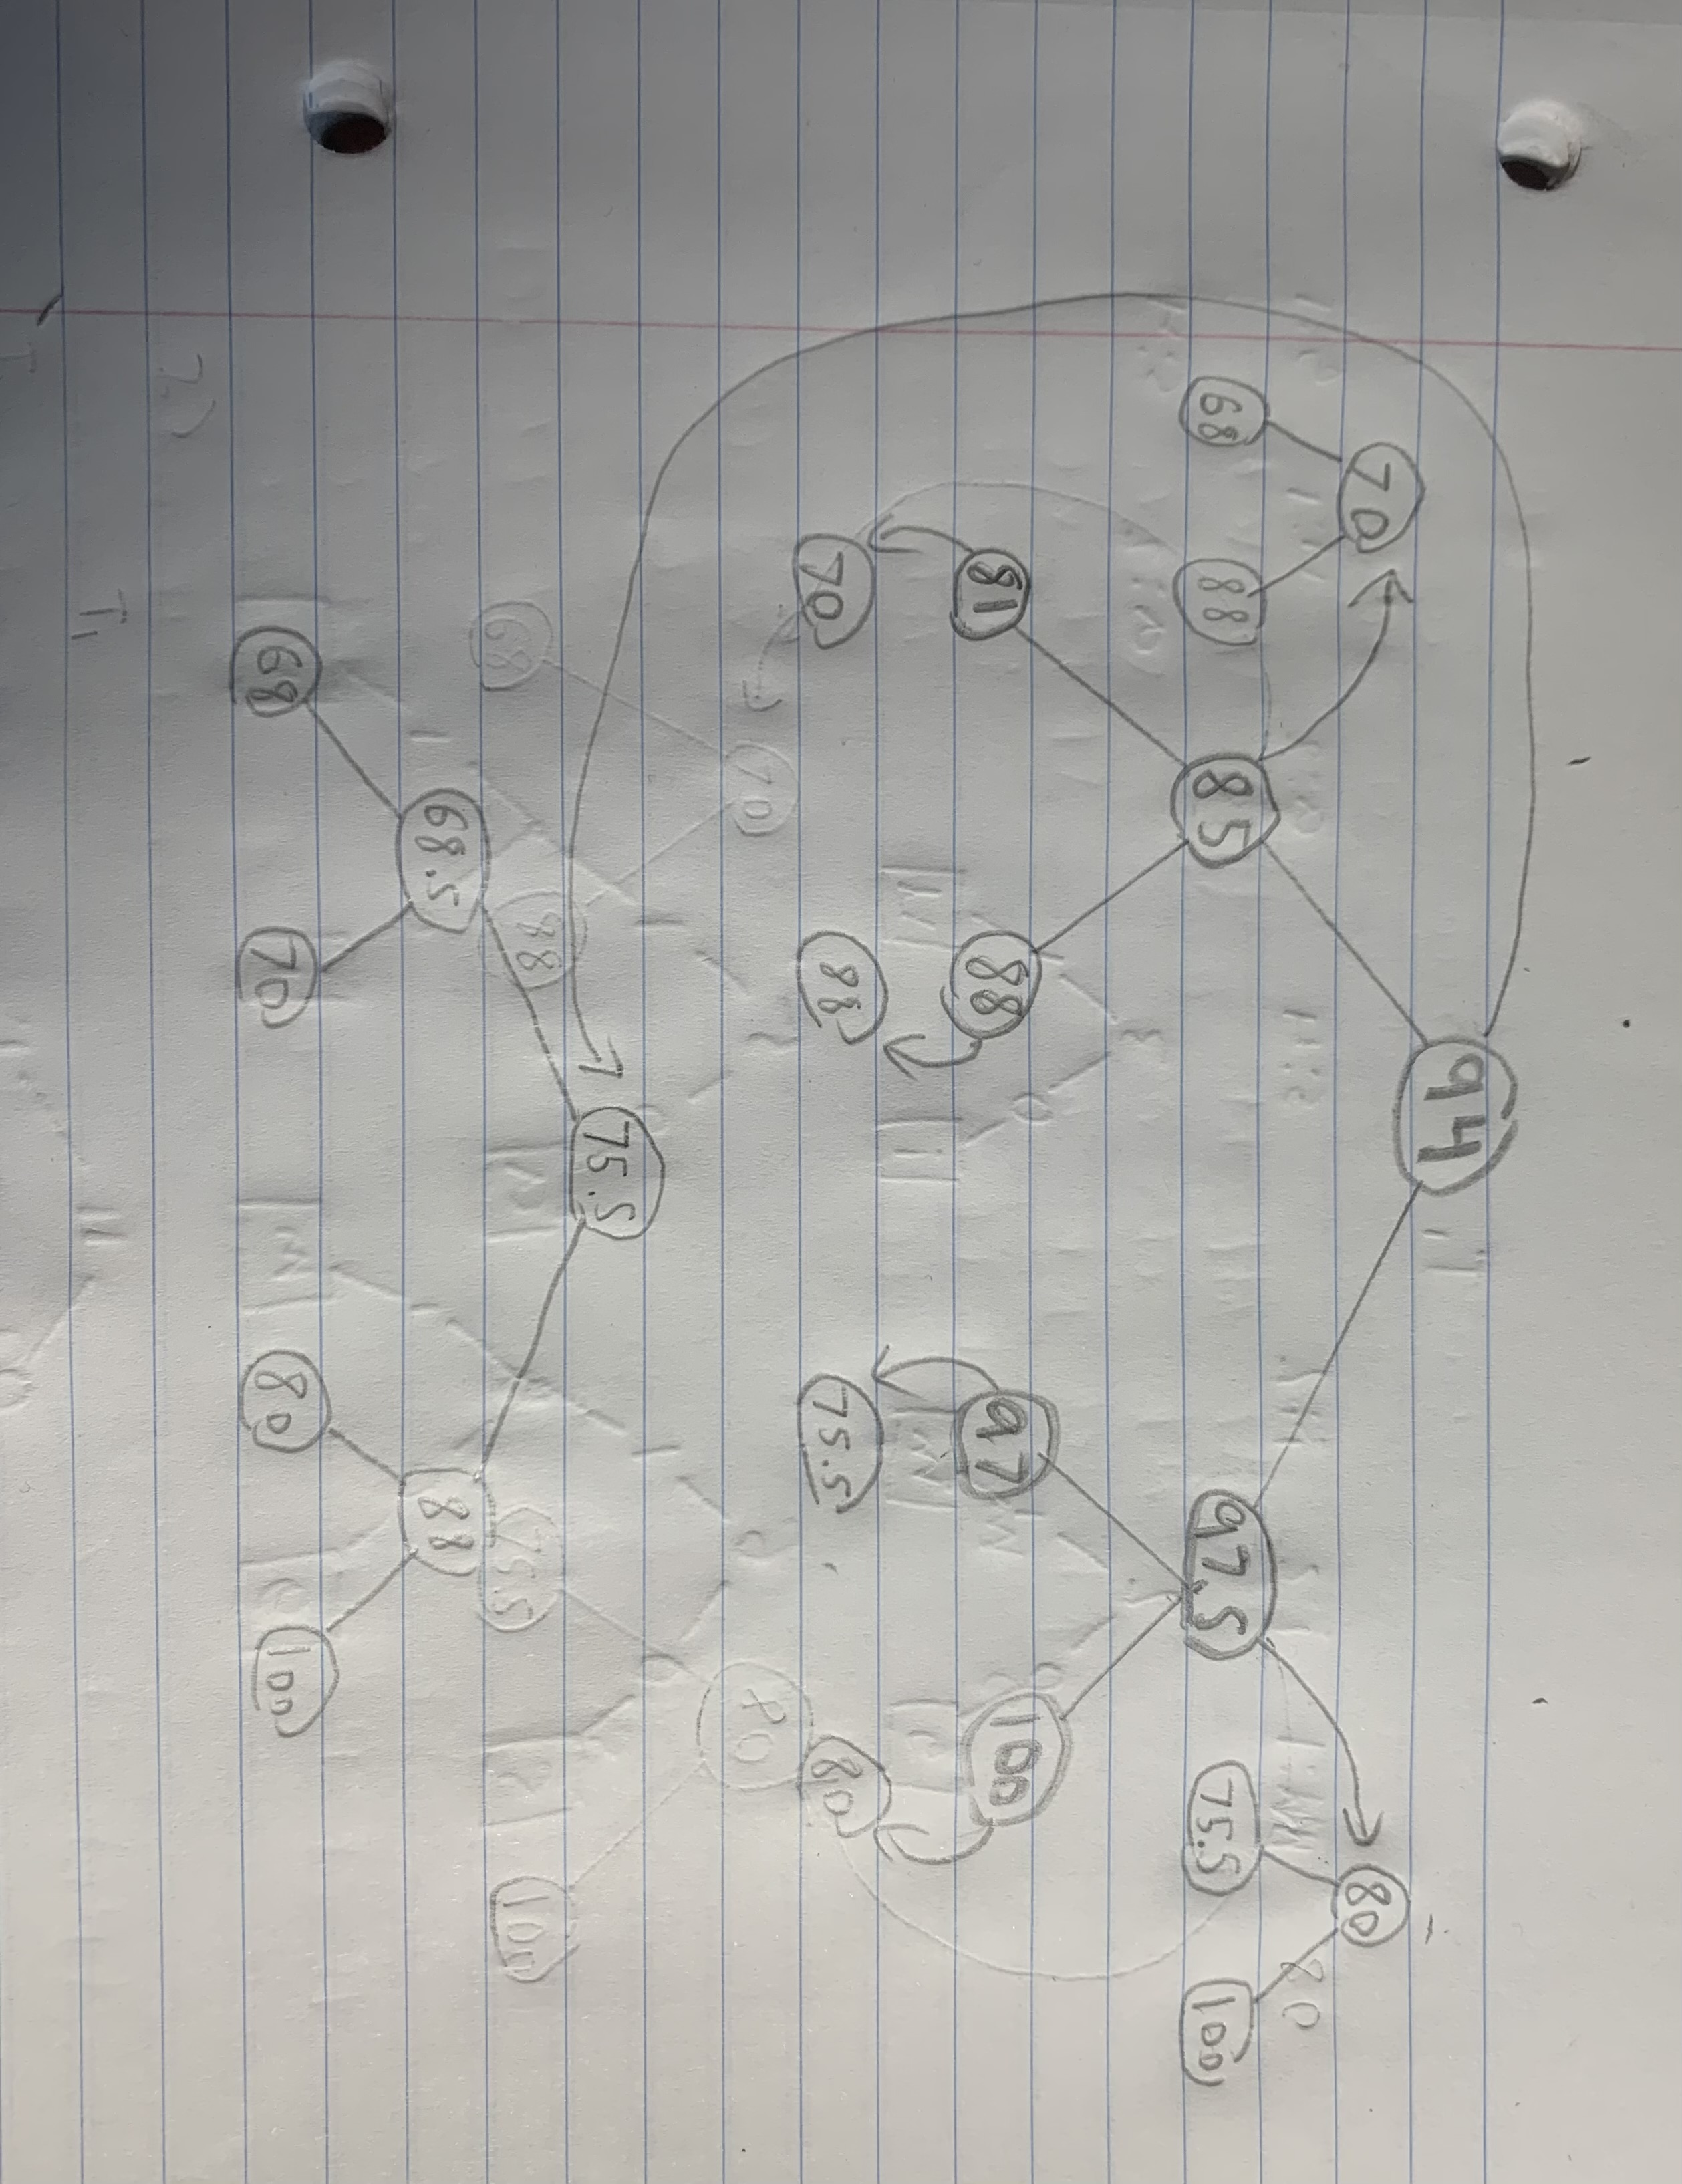
\includegraphics[width=0.8\textwidth, angle=90]{p1.jpg}
	\end{center}
\end{figure}
\end{adjustwidth} 
\newpage
\begin{adjustwidth}{0em}{0pt}
\textbf{Q4b)} Assume that we have a set of $n$ numbers (not necessarily integers) and we are interested only
in the number of points that lie in a range rather than in reporting all of them. Describe how a 1-dimensional range tree (i.e., a balanced BST) can be modified such that a range counting query can be performed in $O(\log n)$ time (independent of $s$).  Briefly justify that your algorithm is within the expected run-time. \\\\
To produce this query we will update each node such that it store the number of child nodes that it has. For the range query we will search for all values between [i,j], where both $i$ and $j$. Because of our modifications, the root node will now store the number of nodes in the tree so we can access and store it a variable called {\tt num\_elements} in O(1) time. We will then do two queries:\\\\
The first query will find the number of elements that are strictly less then i. For each node, if the value of the node is less then or equal to $i$ (i.e we are to the left of the lower bound) we know that all the children to the left of our current node will be less then the lower bound and thus not in the range. Therefore we will subtract {\tt num\_elements} by the number of child elements in the nodes left child. If the node is equal not $i$ we will subtract {\tt num\_elements} by additional 1. In either case we will finish by recursing on the right node.\\ If the node is greater then $i$ then we will recurse on the left child node.\\\\
The second query will find the number of elements that are strictly greater then i. For each node if the value of the node is greater then $j$ we will subtract {\tt num\_elements} by the number of child elements in the nodes right child and by an additional 1 (to represent the current node also not being in the range), and then recurse on the left child. Otherwise if the node is equal to $j$ we will subtract {\tt num\_elements} by the number of child elements in the nodes right child. Otherwise we will recuse on the right child node.\\\\
Note that for each query, each node will either recurse on the left child node or the right child node but never both. Therefore each query at maximum will recurse down the height of the tree (which is $log(n)$) thus our run time is given by:
\[ O(1 + log(n) + log(n)) = O(log(n)) \]
\end{adjustwidth} 
\newpage
\begin{adjustwidth}{0em}{0pt}
\textbf{Q4c)} Aext, consider the 2-dimensional case where we have a set of n 2-dimensional points.
Given a query rectangle R, we only want to find the number of points inside R, not
the points themselves. Explain how to modify the Range Tree data structure discussed
in class such that you can answer any of these counting queries in $O((\log n)^2))$ time.
Briefly justify that your algorithm is within the expected run-time. \\\\
To produce this query we will update each node such that it store the number of child nodes that it has. For the range query we will search for all values between [$x_i$,$x_j$] and [$y_i$, $y_j$]. Because of our modifications, the root node will now store the number of nodes in the tree so we can access and store it a variable called {\tt num\_elements} in O(1) time.\\\\ We will reuse the algorithm we created in 4b, we shall call it {\tt 1DRangeSort}, it will take in a tree node and a range, it will then modify {\tt num\_elements} and subtract the number of elements that don't satisfy the range. Our new algorithm will also do two queries on the original tree:\\\\
Much like in 4b, the first query will find the number of elements that are less then $x_i$ and we will use the exact same algorithm (using the x range to compare). However in the case  that the node.x is greater then $i$ (we will call these types of node border nodes), if it is we will call {\tt 1DRangeSort} on its right child (as its an inner most node). We will then check if the associated y value is between [$y_i$, $y_j$], if its not then we will subtract {\tt num\_elements} by 1. We will then recurse on the left child.\\\\
The second query will find the numbers that are greater then $x_j$ and we will use the same algorthim. However if node.x is less then $j$ we will call {\tt 1DRangeSort} on its left child. We will then check if the associated y value is between [$y_i$, $y_j$], if its not then we will subtract {\tt num\_elements} by 1. We will then recurse on the left child.\\\\
If $n$ represents the number of border nodes and $m$ represents the number of inner most nodes our run time is:
\[ n + m*log(n) \]
In the worst case each of the border nodes on the left and right side will have a inner most node (not including the root node. This means that $n = 2log(n) + 1$ and so $m=2log(n)$. And so our recurrence relation becomes:
\[ 2log(n) + 2log(n)*log(n) = O(log(n)*log(n)) \]
\end{adjustwidth} 
\end{document}